\documentclass[../main.tex]{subfiles}

\begin{document}
\قسمت{گیت‌هاب من}

\زیرقسمت{مقدمه}

گیت‌هاب یک سرویس بسیار مشهور در زمینه‌ی نگهداری و نسخه‌بندی کدهای منبع است. بسیاری از شما به صورت روزمره از آن استفاده می‌کنید.
قصد داریم با استفاده از رابط‌های برنامه‌نویسی این سرویس مقداری با آن تعامل کرده و اطلاعات یک کاربر را استخراج کنیم.

\زیرقسمت{وبگاه}

وبگاهی که طراحی می‌کنید، از شِمای شکل \رجوع{fig:high-level-design} پیروی می‌کند. یک پس زمینه تمام صفحه را در بر گرفته است و در میان آن یک مستطیل شفاف قرار گرفته است.
دقت داشته باشید شفافیت نباید به قدری باشد که متن‌های درون مستطیل خوانایی نداشته باشند.
پیشنهاد می‌شود برای جذابیت پروژه از پس‌زمینه‌هایی با موضوع \متن‌لاتین{octcat} که نماد سرویس گیت‌هاب می‌باشد استفاده کنید.

\begin{figure}[h]
  \centering
  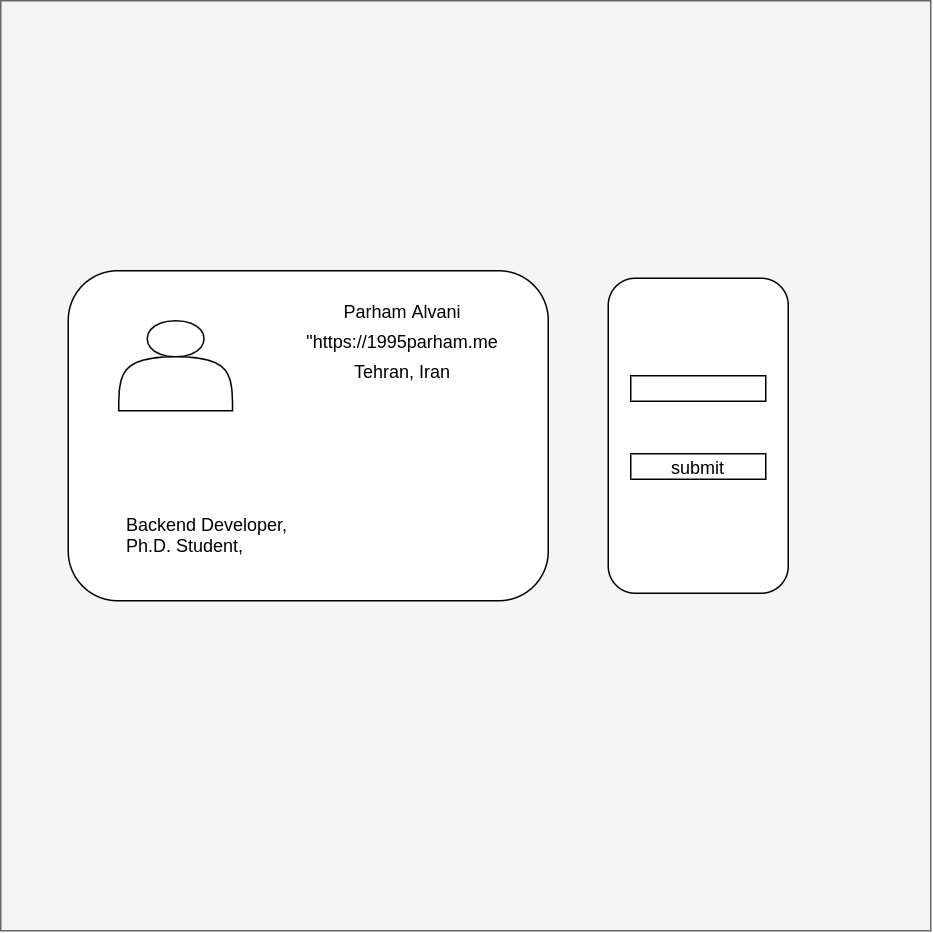
\includegraphics[scale=0.25]{./github}
  \caption{طراحی سطح بالا}
  \label{fig:high-level-design}
\end{figure}

\پاراگراف{}
مستطیل میانی تمامی محتویات قابل نمایش شما را می‌بایست شامل شود. این مستطیل می‌بایست تنها به اندازه محتویات باشد اما برای نمایش زیباتر آن از لایه‌گذاری\پانویس{padding} استفاده کنید.
آنچه در سمت چپ صفحه نمایش داده می‌شود، اطلاعات یک کاربر است که از طریق رابط‌های برنامه‌نویسی استخراج شده است. این اطلاعات شامل تصویر کاربر،
نام کامل کاربر، آدرس بلاگ کاربر، محل زندگی کاربر می‌باشد.
در نهایت پس از این اطلاعات بایو کاربر در یک باکس نمایش داده می‌شود.
تمامی این اطلاعات می‌توانند خالی باشند بنابراین نهایت دقت را برای بررسی این اطلاعات صورت دهید.

در سمت راست صفحه فرمی جهت وارد کردن و ارسال نام کاربری موردنظر در سرویس گیت‌هاب قرار دارد.

\پاراگراف{}
رابط برنامه‌نویسی گیت‌هاب بسیار گسترده می‌باشد. در صورت نیاز می‌توانید از وب‌گاه زیر برای کسب اطلاعات بیشتر استفاده کنید:

\begin{latin}\begin{center}
https://docs.github.com/en/rest/reference
\end{center}\end{latin}

برای کسب اطلاعات یک کاربر می‌توانید یک تقاضا \متن‌لاتین{GET} با ساختار زیر ارسال کنید:

\begin{latin}\begin{center}
https://api.github.com/users/\textit{\{username\}}
\end{center}\end{latin}

با جایگزین کردن یک نام کاربری مثلا \متن‌لاتین{1995parham} پاسخی با ساختار زیر خواهید داشت:
(در نظر داشته باشید بخشی از پاسخ برای کوتاهتر شدن حذف شده است.)

\begin{latin}
\begin{minted}[bgcolor=LightGray]{json}
{
  "login": "1995parham",
  "id": 8181240,
  "node_id": "MDQ6VXNlcjgxODEyNDA=",
  "avatar_url": "https://avatars.githubusercontent.com/u/8181240?v=4",
  "gravatar_id": "",
  "url": "https://api.github.com/users/1995parham",
  "type": "User",
  "site_admin": false,
  "name": "Parham Alvani",
  "company": "@aut-ce @snapp-cab",
  "blog": "https://1995parham.me",
  "location": "Tehran, Iran",
  "email": null,
  "hireable": null,
  "bio": "Backend Developer,\r\nPh.D. Student,\r\nHappy and Smiling",
  "twitter_username": null,
  "public_repos": 80,
  "public_gists": 5,
  "followers": 812,
  "following": 627,
  "created_at": "2014-07-16T14:33:05Z",
  "updated_at": "2021-04-27T04:51:43Z"
}
\end{minted}
\end{latin}

در صورتی که کاربری با نام کاربری داده شده پیدا نشد، می‌بایست پیام خطای مناسبی به کاربر نمایش داده شود.
برای نمایش این پیام از \متن‌لاتین{alert} استفاده نکنید و به طور مثال قسمتی از صفحه را به نمایش آن اختصاص دهید.

\شروع{امتیازی}
همانطور که حدس می‌زنید این اطلاعات برای یک کاربر کافی نمی‌باشد، یکی از اطلاعات مهم برای شرکت‌ها زبان برنامه‌نویسی شخص می‌باشد.
از طریق مخازن کاربر می‌توان به این اطلاعات دست پیدا کرد، برای مثال در این پروژه ما از این رویه استفاده می‌کنیم:

\شروع{شمارش}
\فقره پنج مخزنی که اخیرا در آن \متن‌لاتین{push} کرده است بدست می‌آوریم.
\فقره زبان‌های این پنج مخزن را بدست می‌آوریم.
\فقره زبانی که بیشتری امتیاز را دارد، زبان مورد علاقه کاربر است.
\پایان{شمارش}
\پایان{امتیازی}

\شروع{امتیازی}
در صورتی که ارسال تقاضا به سرویس‌گیت‌هاب به دلایل شبکه‌ای به مشکل خورد پیام مناسبی روی صفحه نمایش داده شود.
در نظر داشته باشید که این پیام نباید در قالب \متن‌لاتین{alert} باشد.
\پایان{امتیازی}

\پاراگراف{}
همانطور که شاید خودتان نیز توجه کرده باشید در قسمت \متن‌لاتین{bio} رشته‌ای که دریافت می‌کنید شامل کاراکترهایی مانند \متن‌لاتین{newline} می‌باشد. برای نمایش صحیح این قسمت می‌بایست فکری بکنید.
در رابطه با عکس پروفایل هم شما لینک عکس را دریافت می‌کنید و کافی است آن را به عنوان \متن‌لاتین{src} در یک عنصر \متن‌لاتین{img} قرار دهید.

\زیرقسمت{حافظه موقت}
\پاراگراف{}
همانطور که خودتان نیز حدس می‌زنید استفاده از رابط‌های برنامه‌نویسی گیت‌هاب رایگان نیست و شما تعداد مشخصی تقاضای رایگان در یک بازه مشخص می‌توانید داشته
باشید. می‌خواهیم با استفاده از یک حافظه موقت جلو تقاضاهای تکراری به این سرویس را بگیریم. شما می‌بایست بعد از هر تقاضا اطلاعات مورد نیاز شخص که پیشتر
بیان شد را در قالب کوکی در مرورگر ذخیره کنید و اگر دوباره برای همان نام‌کاربری تقاضا ارسال شد محتویات از داخل حافظه موقت نمایش داده شوند.
برای درک بهتر کاربر زمانی که اطلاعات از حافظه موقت استخراج می‌شوند یک پیام مناسب نمایش داده خواهد شد.

\شروع{امتیازی}
می‌توانید به جای استفاده از کوکی‌ها از \متن‌لاتین{local storage} استفاده کنید. برای آشنایی بیشتر می‌توانید از وبگاه زیر کمک بگیرید.


\begin{latin}\begin{center}
https://developer.mozilla.org/en-US/docs/Web/API/Window/localStorage
\end{center}\end{latin}

\پایان{امتیازی}

\زیرقسمت{نکات پیاده‌سازی}

\شروع{فقرات}
    \فقره برای کدهایتان از کامنت استفاده کنید. توضیح کارکرد بلاک‌های \متن‌لاتین{CSS} اجباری می‌باشد. توابعی و قطعات کد جاوا اسکریپت نیز می‌بایست حداقل یک خط کامنت داشته باشند.
    \فقره کامنت فارسی یا انگلیسی موردی ندارد اما از فینگلیش (!) نوشتن پرهیز کنید.
    \فقره استفاده از کتابخانه‌ها و چهارچوب‌ها در پروژه مجاز \متن‌سیاه{نمی‌باشد}.
    \فقره از آنجایی که این پروژه در قالب \متن‌سیاه{امتحان میانترم} می‌باشد از تغییر دادن صورت مساله یا انجام موارد خارج از موارد مطرح شده خودداری کنید.
    \فقره در نظر داشته باشید نمره پروژه و قسمت امتیازی آن محدود است اما موارد امتیازی زیادی می‌توان به آن اضافه کرد، بنابراین از گذاشتن زمان بیشتر از حد معمول برای پروژه خودداری کنید.
\پایان{فقرات}

\زیرقسمت{پرسش‌های متداول}

صورت پروژه در مهلت انجام پروژه بر پایه سوالات شما به روزرسانی خواهد شد.
\شروع{توضیح}
\فقره[پرسش (۱)] آیا استفاده از کتابخانه‌ی \متن‌لاتین{bootstrap} مجاز است؟
\فقره[پاسخ] خیر مجاز \متن‌سیاه{نمی‌باشد}.
\فقره[پرسش (۲)] آیا هندل کردن خطا اجباری است یا امتیازی؟
\فقره[پاسخ] هندل کردن خطای ناشی از وجود نداشتن یک نام کاربری اجباری است اما هندل کردن خطای شبکه امتیازی می‌باشد.
\فقره[پرسش (۳)] آیا ذخیره کردن آدرس عکس کافی است؟
\فقره[پاسخ] بله محدودیت گیت‌هاب به صورت مشخص روی رابط برنامه‌نویسی بسیار سخت‌گیرانه‌تر از رابط دریافت عکس‌ها می‌باشد پس ذخیره آدرس عکس کافی است.
\پایان{توضیح}

\end{document}
